\documentclass[11pt]{article}

% some definitions for the title page
\newcommand{\reporttitle}{Pre-training Models}
\newcommand{\reportdescription}{Includes topics such as contextual word representations, pre-training encoder models, BERT and relatives and pre-training encoder-decoder models.}

% load some definitions and default packages
%---------------------------------------------------------------------------
%	PACKAGES AND OTHER DOCUMENT CONFIGURATIONS
%---------------------------------------------------------------------------

\usepackage[twoside]{fancyhdr}
\usepackage{csquotes}

\usepackage[a4paper,hmargin=2.0cm,vmargin=1.0cm,includeheadfoot]{geometry}
% \usepackage{natbib} % for bibliography
\usepackage{biblatex}
\usepackage{tabularx,longtable,multirow,subfigure,caption}%hangcaption
\usepackage{fancyhdr} % page layout
\usepackage{url} % URLs
\usepackage[english]{babel}
\usepackage{amsmath}
\usepackage{graphicx}
\usepackage{dsfont}
\usepackage{epstopdf} % automatically replace .eps with .pdf in graphics
% \usepackage{backref} % needed for citations
\usepackage{array}
\usepackage{latexsym}
\usepackage[pdftex,hypertexnames=false,colorlinks]{hyperref} % provide links in pdf (had pagebackref)
\usepackage{booktabs}
\usepackage{wrapfig}
\usepackage{caption}  % Required for \captionof
\usepackage{float} % for H option in figures
\usepackage{amssymb}
\usepackage{amsmath}
\usepackage[nottoc]{tocbibind}

%%% Default fonts
\renewcommand*{\rmdefault}{bch}
\renewcommand*{\ttdefault}{cmtt}

%%% Default settings (page layout)
\setlength{\parindent}{0em}  % indentation of paragraph
\setlength{\parskip}{.3em}

\setlength{\headheight}{14.5pt}
\pagestyle{fancy}

\fancyfoot[ER,OL]{\thepage}%Page no. in the left on odd pages and on right on even pages

\fancyfoot[OC,EC]{\sffamily }
\renewcommand{\headrulewidth}{0.1pt}
\renewcommand{\footrulewidth}{0.1pt}
\captionsetup{margin=10pt,font=small,labelfont=bf}
% Here, you can define your own macros. Some examples are given below.

\newcommand{\R}[0]{\mathds{R}} % real numbers
\newcommand{\Z}[0]{\mathds{Z}} % integers
\newcommand{\N}[0]{\mathds{N}} % natural numbers
\newcommand{\C}[0]{\mathds{C}} % complex numbers
\renewcommand{\vec}[1]{{\boldsymbol{{#1}}}} % vector
\newcommand{\mat}[1]{{\boldsymbol{{#1}}}} % matrix

\usepackage{pifont,mdframed}
\newenvironment{warning}
  {\par\begin{mdframed}[linewidth=1pt,linecolor=black]%
    \begin{list}{}{\leftmargin=1cm
                   \labelwidth=\leftmargin}\item[\Large\ding{43}]}
  {\end{list}\end{mdframed}\par}

%\bibliography{bibliography}

\begin{document}

% Include the title page
\begin{titlepage}

    \newcommand{\HRule}{\rule{\linewidth}{0.5mm}} % Defines a new command for the horizontal lines, change thickness here
    
    \center % Center everything on the page
     
    %------------------------------------------------------------------------
    %	HEADING SECTIONS
    %------------------------------------------------------------------------
    
    \textsc{\Large Department of Computing}\\[0.5cm] 
    \textsc{\large Imperial College of Science, Technology and Medicine}\\[0.5cm] 
    
    %------------------------------------------------------------------------
    %	TITLE SECTION
    %------------------------------------------------------------------------
    
    \HRule \\[0.4cm]
    { \huge \bfseries \reporttitle}\\ % Title of your document
    \HRule \\[0.4cm]

    \textit{\reportdescription}
    
    \vspace{2em}

    %------------------------------------------------------------------------
    %	AUTHOR SECTION
    %------------------------------------------------------------------------
    
    \large \emph{Author: Anton Zhitomirsky}

    \vspace{1em}

    \global\let\newpagegood\newpage
    \global\let\newpage\relax
    
\end{titlepage}

\global\let\newpage\newpagegood


\begin{figure}[H]
    \centering
    \subfigure{\fbox{\includegraphics[page=3, trim=1.1cm .5cm 1.5cm 2cm, clip, width=.45\linewidth]{Lecture 6.2 - Pre-training models.pdf}}}
\end{figure}    



\tableofcontents

\clearpage

\section{Contextual Word Representations}

Word Embeddings allow us to learn vector representations for individual words, useful for applications such as representing similar words with similar vectors, synonym replacement, word classification and so on. However, their shortcoming is that each word has only one embedding, and often times the meaning of a word depends on the context.

For instance, an example:

\begin{quote}
    I deposited some money in the \emph{bank} VS I was camping on the east \emph{bank} of the river.
\end{quote}

Here,having a single vector for every word doesn't cut it since we need to take the context into account when constructing word representations.

\subsection{RNN}

\begin{figure}[H]
    \centering
    \subfigure{\fbox{
\includegraphics[page=6, trim=1.5cm .5cm 1.5cm 6.5cm, clip, width=.95\linewidth]{Lecture 6.1 - Pre-training models.pdf}}}
    \caption*{One way, is to use a model like an RNN; by going through the text in sequence and building up representations of the text, you can use them for word representations as well. Internally, it will learn to encode any given context into a vector.}
\end{figure}    

\subsection{ELMo}

\begin{minipage}[l]{.5\linewidth}
    \begin{figure}[H]
        \centering
        \subfigure{\fbox{
\includegraphics[page=7, trim=1.5cm 3cm 4cm 3cm, clip, width=.95\linewidth]{Lecture 6.1 - Pre-training models.pdf}}}
    \end{figure}    
\end{minipage}\hfill
\begin{minipage}[r]{.48\linewidth}
    Embeddings from Language Models:
    \begin{itemize}
        \item One model tries to predict the next word and another tries to predict the previous word in the sentence.
        \item The two are trained on large volumes of text.
    \end{itemize}
\end{minipage}

\begin{figure}[H]
    \centering
    \subfigure{\fbox{
\includegraphics[page=8, trim=1.5cm 2cm 1.5cm 7cm, clip, width=.8\linewidth]{Lecture 6.1 - Pre-training models.pdf}}}
    \caption*{The idea is to take the embeddings from both directions and combine them into one vector representation}
\end{figure}    

\subsubsection{Architecture}

\begin{minipage}[l]{.5\linewidth}
    \begin{figure}[H]
        \centering
        \subfigure{\fbox{
\includegraphics[page=9, trim=1.5cm .5cm 1.5cm 2cm, clip, width=.95\linewidth]{Lecture 6.1 - Pre-training models.pdf}}}
    \end{figure}    
\end{minipage}\hfill
\begin{minipage}[r]{.48\linewidth}
    \begin{itemize}
        \item ELMo uses LSTMS as opposed to regular rnns.
        \item They have multiple layers of LSTMS
        \item If a sentence is given, it is embedded and fed into a bidirectional LSTM, which then gets fed into the next layer again.
        \item The final vector gets combined from all the layers.
    \end{itemize}
\end{minipage}

Having multiple layers allows for more complex `second-level' reasoning about words.

\begin{figure}[H]
    \centering
    \subfigure{\fbox{
\includegraphics[page=10, trim=1.1cm .5cm 1.5cm 2cm, clip, width=.45\linewidth]{Lecture 6.1 - Pre-training models.pdf}}}
\end{figure}    

\section{BERT}

\begin{minipage}[l]{.5\linewidth}
    \begin{figure}[H]
        \centering
        \subfigure{\fbox{
\includegraphics[page=12, trim=.8cm .5cm 1.5cm 1.51cm, clip, width=.95\linewidth]{Lecture 6.1 - Pre-training models.pdf}}}
    \end{figure}    
\end{minipage}\hfill
\begin{minipage}[r]{.48\linewidth}
    \begin{itemize}
        \item ELMo was the first important model of this type
        \item Nowadays, we have three different types of models.
        \item Decoders are efficient: the bounding of reading to the left makes it more technically efficient than an encoder; each time you generate a new word you don't want to recalculate the context representations for the whole context. Instead, you attend only to the left.
    \end{itemize}
\end{minipage}

\begin{minipage}[l]{.5\linewidth}
    \begin{figure}[H]
        \centering
        \subfigure{\fbox{
\includegraphics[page=13, trim=13cm 2cm 1.5cm 3cm, clip, width=.8\linewidth]{Lecture 6.1 - Pre-training models.pdf}}}
    \end{figure}    
\end{minipage}\hfill
\begin{minipage}[r]{.48\linewidth}
    Bidirectional Encoder Representations from Transformers
    \begin{itemize}
        \item Takes in a sequence of tokens, gives as output a vector for each token. At the output it produces the same number of representations as tokens in the input.
        \item Builds on previous word (ELMo) and combines some good ideas and scales it up further.
    \end{itemize}
\end{minipage}

\subsection{What is inside the transformer encoder?}

\begin{minipage}[l]{.5\linewidth}
    \begin{figure}[H]
        \centering
        \subfigure{\fbox{
\includegraphics[page=14, trim=1.1cm .5cm 1.5cm 2cm, clip, width=.95\linewidth]{Lecture 6.1 - Pre-training models.pdf}}}
    \end{figure}    
\end{minipage}\hfill
\begin{minipage}[r]{.48\linewidth}
    \begin{itemize}
        \item A transformer cell/layer takes words as input through the bottom. 
        \item This cell is repeated as many times as we like.
    \end{itemize}
\end{minipage}

\subsubsection{Self-attention}

\begin{figure}[H]
    \centering
    \subfigure[Bert uses self attention | every word in the sequence calculates new representations based on all the other words in the sequence.]{\fbox{
\includegraphics[page=15, trim=1.1cm .5cm 1.5cm 2cm, clip, width=.45\linewidth]{Lecture 6.1 - Pre-training models.pdf}}}
    \subfigure[Advantage from self-attention is that every word is just one hop away from every other word. In LSTMs or RNNs, if we wanted to get infromation from one word to another, we'd ahve to step through every word in the sequence and keep information in memory. Unlike Self-attention which combines directly infromatino from every other word.]{\fbox{
\includegraphics[page=16, trim=1.1cm .5cm 1.5cm 2cm, clip, width=.45\linewidth]{Lecture 6.1 - Pre-training models.pdf}}}
\end{figure}    

\subsubsection{Multi-head self-attention}

\begin{minipage}[l]{.5\linewidth}
    \begin{figure}[H]
        \centering
        \subfigure{\fbox{
\includegraphics[page=17, trim=1.1cm .5cm 1.5cm 2cm, clip, width=.95\linewidth]{Lecture 6.1 - Pre-training models.pdf}}}
    \end{figure}    
\end{minipage}\hfill
\begin{minipage}[r]{.48\linewidth}
    \begin{itemize}
        \item Each head is able to specialize to a particular task
        \item e.g. one head might be doing who, another, did what, another to whom. (we don't know, we let it learn whatever it needs to)
        \item Then, all this is combined into one representation.
    \end{itemize}
\end{minipage}

\subsubsection{Input embeddings}

\begin{minipage}[l]{.5\linewidth}
    \begin{figure}[H]
        \centering
        \subfigure{\fbox{
\includegraphics[page=19, trim=1.1cm .5cm 1.5cm 3cm, clip, width=.95\linewidth]{Lecture 6.1 - Pre-training models.pdf}}}
    \end{figure}    
\end{minipage}\hfill
\begin{minipage}[r]{.48\linewidth}
    \begin{itemize}
        \item We tokenize an input sentence
        \item \textbf{Token Embeddings}: normal learnable embeddings learnt during the training of the BERT model
        \item \textbf{Segment Embeddings}: shows the model where in the input a word is, specifically, which section.
        \item \textbf{Position Embeddings}: positional predefined sinosoidal embeddings or learnable embeddings.
    \end{itemize}
\end{minipage}

\subsection{Training}

\subsubsection{Masked Language Modelling}

How do we train our model? We want it to have as much training data as possible so that is learns as much as it can. For that, we would want to use just plain text because annotated data is very expensive to obtain. Furthermore, there is not that much available versus all the data on the internet that you can crawl.

\begin{figure}[H]
    \centering
    \subfigure{\fbox{
\includegraphics[page=20, trim=1cm 1cm 1.3cm 8.5cm, clip, width=.95\linewidth]{Lecture 6.1 - Pre-training models.pdf}}}
    \caption*{Here, the language model learns to predict missing words. We Hide $k\%$ of the input words behind a mask and train the model to predict them. Since BERT returns a representation for each token, we only train those parts for which a word is absent.}
\end{figure}    

\begin{minipage}[l]{.5\linewidth}
    \begin{figure}[H]
        \centering
        \subfigure{\fbox{
\includegraphics[page=22, trim=1.1cm .5cm 1.5cm 2cm, clip, width=.95\linewidth]{Lecture 6.1 - Pre-training models.pdf}}}
    \end{figure}    
\end{minipage}\hfill
\begin{minipage}[r]{.48\linewidth}
    \begin{itemize}
        \item When we train these models we want the correct amount of masking. 
        \item When we have too little masking, the model needs to consider the entire scope of the document to make a prediction. 
        \item if we have too much masking, then we may just lack enough information to fill in the gap correctly.
    \end{itemize}
\end{minipage}

The last two bullet points are curious. We replace 10\% with random words because in basic training it won't ever have any incorrect words. This trains the model to calculate correct representations regardless of the context which has varying truth. Then, 10\% is left as the original but also predicted because if we train the model to only predict correct words where there is a mask token, then the model will learn to only predict in those places; in practice we don't have any masks.

\subsubsection{Next sentence prediction}

BERT used a second pre-training objective. It is given two sentences, and it tries to predict whether they appeared in the original order in the source text. However, this didn't add much benefit so it hasn't been used in newer versions.

\begin{figure}[H]
    \centering
    \subfigure{\fbox{
\includegraphics[page=23, trim=1.1cm 4.5cm 1.5cm 7cm, clip, width=.95\linewidth]{Lecture 6.1 - Pre-training models.pdf}}}
\end{figure}    

\subsection{Variants}

\begin{figure}[H]
    \centering
    \subfigure{\fbox{
\includegraphics[page=24, trim=1.1cm .5cm 1.5cm 2cm, clip, width=.45\linewidth]{Lecture 6.1 - Pre-training models.pdf}}}
\end{figure}    

\section{Putting pre-trained models to work}

BERT-like models give us a representation vector for every input token. We just have to chop off the masked LM head, it is no longer needed.

We can use those vectors to represent individual tokens or full sentences

\begin{enumerate}
    \item Freeze BERT, use it to calculate informative representation vectors. Train another ML model that uses these vectors as input.
    \item (more commonly) Put a minimal neural architecture on top of BERT (e.g. a single output layer). Train the whole thing end-to-end (called fine-tuning)
\end{enumerate}

\begin{figure}[H]
    \centering
    \subfigure[For \textbf{sentence classifcation}, give the language to BERT and attach it to an output layer to predict a lable. If BERT produces tokens for every token, we attach our layer to the CLS token so that the model produces good text representations as that token's representation; \textbf{Add a special token in the input that represents the whole sentence}]{\fbox{
\includegraphics[page=27, trim=7.5cm .5cm 6.5cm 3.6cm, clip, width=.45\linewidth]{Lecture 6.1 - Pre-training models.pdf}}}
    \subfigure[\textbf{Token Labelling}: assigning labels to individual tokens, do the same, just put classifciations pairs on each token.]{\fbox{
\includegraphics[page=28, trim=7.5cm .5cm 6.5cm 3.6cm, clip, width=.45\linewidth]{Lecture 6.1 - Pre-training models.pdf}}}
    \subfigure[\textbf{Pair Classification}: we separate two sentences with a token.  We put a classification head on top of the class token and train the model to classify `does sentence 1 entail sentence 2 or vice versa'?]{\fbox{
\includegraphics[page=29, trim=8cm .5cm 6cm 3.6cm, clip, width=.45\linewidth]{Lecture 6.1 - Pre-training models.pdf}}}
    \subfigure[\textbf{Question Answering}: We can structure the task with an input, and a paragraph of text which may contain some answers. Then train the model to lable individual tokens to indicate which tokens are the answer, then simply extract these.]{\fbox{
\includegraphics[page=30, trim=7.5cm .5cm 6.5cm 3.6cm, clip, width=.45\linewidth]{Lecture 6.1 - Pre-training models.pdf}}}
\end{figure}    

\subsection{Performance}

\begin{figure}[H]
    \centering
    \subfigure{\fbox{
\includegraphics[page=31, trim=1.1cm 5cm 1.4cm 4.3cm, clip, width=.95\linewidth]{Lecture 6.1 - Pre-training models.pdf}}}
\end{figure}    

\textbf{QQP, STS-B, MRPC}: Detecting similar text and paraphrases
\textbf{QNLI, RTE}: Detecting entailment (natural language inference)
\textbf{SST-2}: Sentiment analysis (positive / negative / neutral)
\textbf{CoLA}: Detecting grammaticality of text

\section{Text classification with BERT in practice}

\begin{figure}[H]
    \centering
    \subfigure{\fbox{
\includegraphics[page=33, trim=1.1cm .5cm 1.5cm 2cm, clip, width=.45\linewidth]{Lecture 6.1 - Pre-training models.pdf}}}
    \caption*{\href{https://huggingface.co/}{hugging face} is a website with many pre-trained models}
\end{figure}    

\subsection{Worked Example}

This example lives on \href{https://github.com/marekrei/bert_text_classification_example}{Marke's Github}

\begin{figure}[H]
    \centering
    \subfigure{\fbox{
\includegraphics[page=36, trim=1.1cm .5cm 1.5cm 2cm, clip, width=.9\linewidth]{Lecture 6.1 - Pre-training models.pdf}}}
    \subfigure{\fbox{
\includegraphics[page=37, trim=1.1cm .5cm 1.5cm 2cm, clip, width=.9\linewidth]{Lecture 6.1 - Pre-training models.pdf}}}
    \subfigure{\fbox{
\includegraphics[page=35, trim=1.1cm .5cm 1.5cm 2cm, clip, width=.9\linewidth]{Lecture 6.1 - Pre-training models.pdf}}}
\end{figure}    

\section{BERT Variations}

\subsection{BERT $\vert$ RoBERTa $\vert$ DeBERTa}

\begin{figure}[H]
    \centering
    \subfigure{\fbox{
\includegraphics[page=39, trim=1.1cm .5cm 1.5cm 2cm, clip, width=.95\linewidth]{Lecture 6.1 - Pre-training models.pdf}}}
\end{figure}    

\subsection{SpanBERT}

\begin{minipage}[l]{.5\linewidth}
    \begin{figure}[H]
        \centering
        \subfigure{\fbox{
\includegraphics[page=40, trim=1.1cm .5cm 1cm 2cm, clip, width=.95\linewidth]{Lecture 6.1 - Pre-training models.pdf}}}
    \end{figure}    
\end{minipage}\hfill
\begin{minipage}[r]{.48\linewidth}
    \begin{itemize}
        \item They make the task more difficult, and mask out sequences of words. Gives models more incentive to learn more detailed representations.
    \end{itemize}
\end{minipage}

\subsection{DistilBERT $\vert$ ALBERT}

\begin{minipage}[l]{.5\linewidth}
    \begin{figure}[H]
        \centering
        \subfigure{\fbox{
\includegraphics[page=41, trim=1.1cm .5cm 1.5cm 2cm, clip, width=.95\linewidth]{Lecture 6.1 - Pre-training models.pdf}}}
    \end{figure}    
\end{minipage}\hfill
\begin{minipage}[r]{.48\linewidth}
    \begin{itemize}
        \item Sometime models require a lot of resources, and these models return results quickly. E.g. DistilBERT trains a smaller transformer model on the output of the bigger model. 
    \end{itemize}
\end{minipage}

\subsection{BigBird $\vert$ LongFormer}

\begin{minipage}[l]{.5\linewidth}
    \begin{figure}[H]
        \centering
        \subfigure{\fbox{
\includegraphics[page=42, trim=1.1cm .5cm 1.5cm 2cm, clip, width=.95\linewidth]{Lecture 6.1 - Pre-training models.pdf}}}
    \end{figure}    
\end{minipage}\hfill
\begin{minipage}[r]{.48\linewidth}
    \begin{itemize}
        \item Sometimes we need more context. These encode longer text. 
        \item This model attends to some words based on a pattern, e.g. randomly, nearby, or global (some words attend to all, and some don't)
    \end{itemize}
\end{minipage}

\subsection{ClinicalBert $\vert$ MedBert $\vert$ PubMedBert $\vert$ BEHRT}

\begin{minipage}[l]{.5\linewidth}
    \begin{figure}[H]
        \centering
        \subfigure{\fbox{
\includegraphics[page=43, trim=1.1cm .5cm 1.5cm 2cm, clip, width=.95\linewidth]{Lecture 6.1 - Pre-training models.pdf}}}
    \end{figure}    
\end{minipage}\hfill
\begin{minipage}[r]{.48\linewidth}
    \begin{itemize}
        \item Domain specific BERTs also exist. 
        \item There is a specific embedding for the age of the patient, and the segment embeddings for hospital visits.
    \end{itemize}
\end{minipage}

\subsection{ERNIE}

\begin{minipage}[l]{.5\linewidth}
    \begin{figure}[H]
        \centering
        \subfigure{\fbox{
\includegraphics[page=44, trim=1.1cm .5cm 1.5cm 2cm, clip, width=.95\linewidth]{Lecture 6.1 - Pre-training models.pdf}}}
    \end{figure}    
\end{minipage}\hfill
\begin{minipage}[r]{.48\linewidth}
    \begin{itemize}
        \item ``We can have databses and knowledge graphs that contain a lot of factual information and it would be useful to include those in language models as well. So there are models that have been proposed to include this information in BERT by retrieveing relevant infromation from a knoweldge graph, embedding it, and then conecting it directly into the embeddings of BERT.''
    \end{itemize}
\end{minipage}

\subsection{Multi-Lingual Models}

\begin{minipage}[l]{.5\linewidth}
    \begin{figure}[H]
        \centering
        \subfigure{\fbox{
\includegraphics[page=45, trim=1.1cm .5cm 1.5cm 2cm, clip, width=.95\linewidth]{Lecture 6.1 - Pre-training models.pdf}}}
    \end{figure}    
\end{minipage}\hfill
\begin{minipage}[r]{.48\linewidth}
    \begin{itemize}
        \item There are also BERTs for every different language
        \item M-BERt is multilingual
    \end{itemize}
\end{minipage}

\subsection{Multi-Modal Models}

\begin{minipage}[l]{.5\linewidth}
    \begin{figure}[H]
        \centering
        \subfigure{\fbox{
\includegraphics[page=46, trim=1.1cm .5cm 1.5cm 2cm, clip, width=.95\linewidth]{Lecture 6.1 - Pre-training models.pdf}}}
    \end{figure}    
\end{minipage}\hfill
\begin{minipage}[r]{.48\linewidth}
    \begin{itemize}
        \item Where the model can process information both from the visual and textual domain.
    \end{itemize}
\end{minipage}

\subsubsection{ImageBERT}

\begin{minipage}[l]{.5\linewidth}
    \begin{figure}[H]
        \centering
        \subfigure{\fbox{
\includegraphics[page=47, trim=1.1cm .5cm .5cm 2cm, clip, width=.95\linewidth]{Lecture 6.1 - Pre-training models.pdf}}}
    \end{figure}    
\end{minipage}\hfill
\begin{minipage}[r]{.48\linewidth}
    \begin{itemize}
        \item It gets the input text and image, and extracts these little areas from the image that represent different objects. Then encodes these into vectors and maps the into the same space as the textual tokens.
        \item Then we can have multiple different objectives for this task for training.
    \end{itemize}
\end{minipage}

\subsubsection{ViLBERT}

\begin{minipage}[l]{.5\linewidth}
    \begin{figure}[H]
        \centering
        \subfigure{\fbox{
\includegraphics[page=48, trim=1.1cm .5cm 1.5cm 2cm, clip, width=.95\linewidth]{Lecture 6.1 - Pre-training models.pdf}}}
    \end{figure}    
\end{minipage}\hfill
\begin{minipage}[r]{.48\linewidth}
    \begin{itemize}
        \item Contains cross attention models
    \end{itemize}
\end{minipage}

\subsection{Masked image modelling}

\begin{minipage}[l]{.5\linewidth}
    \begin{figure}[H]
        \centering
        \subfigure{\fbox{
\includegraphics[page=49, trim=1.1cm .5cm 1.5cm 2cm, clip, width=.95\linewidth]{Lecture 6.1 - Pre-training models.pdf}}}
    \end{figure}    
\end{minipage}\hfill
\begin{minipage}[r]{.48\linewidth}
    \begin{itemize}
        \item mask different parts of the image and apply mask fixes onto the image.
    \end{itemize}
\end{minipage}

\subsection{Masked protein modelling}

\begin{figure}[H]
    \centering
    \subfigure{\fbox{
\includegraphics[page=50, trim=1.1cm .5cm 1.5cm 2cm, clip, width=.45\linewidth]{Lecture 6.1 - Pre-training models.pdf}}}
\end{figure}    

\section{Pre-training encoder-decoder models}

\subsection{Pipeline}

\begin{minipage}[l]{.5\linewidth}
    \begin{figure}[H]
        \centering
        \subfigure{\fbox{
\includegraphics[page=53, trim=1.1cm .5cm 1.5cm 2cm, clip, width=.95\linewidth]{Lecture 6.1 - Pre-training models.pdf}}}
    \end{figure}    
\end{minipage}\hfill
\begin{minipage}[r]{.48\linewidth}
    \begin{itemize}
        \item We have an encoded part and decoded part
        \item For the encoder, we have the familiar BERT strategy of giving the whole text as input with self-attention over all tokens in all possible directions
        \item We then get these vector representations out for each token which are the passed to the decoder block and the decoder block generates words one word at a time 
        \item It then puts that word back into its own input and encodes that as the context and tries to predict the next word in the sequence.
    \end{itemize}
\end{minipage}

This architecture is particularly useful in machine translation. Another advantage is that encoder and decoder can have separate vocabularies which abstracts the machine translation task better.

\subsection{Pre-training models}

\begin{figure}[H]
    \centering
    \subfigure{\fbox{
\includegraphics[page=54, trim=1.1cm .5cm 1.5cm 2cm, clip, width=.45\linewidth]{Lecture 6.1 - Pre-training models.pdf}}}
    \subfigure{\fbox{
\includegraphics[page=56, trim=1.1cm .5cm 1.5cm 2cm, clip, width=.45\linewidth]{Lecture 6.1 - Pre-training models.pdf}}}
\end{figure}    

% \begin{minipage}[l]{.5\linewidth}
%     \begin{figure}[H]
%         \centering
%         \subfigure{\fbox{
\includegraphics[page=55, trim=1.1cm .5cm 1.5cm 2cm, clip, width=.95\linewidth]{Lecture 6.1 - Pre-training models.pdf}}}
%     \end{figure}    
% \end{minipage}\hfill
% \begin{minipage}[r]{.48\linewidth}
%     \begin{itemize}
%         \item
%     \end{itemize}
% \end{minipage}



% \begin{minipage}[l]{.5\linewidth}
%     \begin{figure}[H]
%         \centering
%         \subfigure{\fbox{
\includegraphics[page=57, trim=1.1cm .5cm 1.5cm 2cm, clip, width=.95\linewidth]{Lecture 6.1 - Pre-training models.pdf}}}
%     \end{figure}    
% \end{minipage}\hfill
% \begin{minipage}[r]{.48\linewidth}
%     \begin{itemize}
%         \item
%     \end{itemize}
% \end{minipage}

\subsection{Instructional training}

\begin{minipage}[l]{.5\linewidth}
    \begin{figure}[H]
        \centering
        \subfigure{\fbox{
\includegraphics[page=58, trim=1.1cm .5cm 1.5cm 2cm, clip, width=.95\linewidth]{Lecture 6.1 - Pre-training models.pdf}}}
    \end{figure}    
\end{minipage}\hfill
\begin{minipage}[r]{.48\linewidth}
    \begin{itemize}
        \item Take annotated datasets and phrase it to look like a sequence to sequence translation task.
    \end{itemize}
\end{minipage}

\begin{minipage}[l]{.5\linewidth}
    \begin{figure}[H]
        \centering
        \subfigure{\fbox{
\includegraphics[page=59, trim=1.1cm .5cm 1.5cm 2cm, clip, width=.95\linewidth]{Lecture 6.1 - Pre-training models.pdf}}}
    \end{figure}    
\end{minipage}\hfill
\begin{minipage}[r]{.48\linewidth}
    \begin{itemize}
        \item The follow-up work creates more human sounding templates.
    \end{itemize}
\end{minipage}

\begin{minipage}[l]{.5\linewidth}
    \begin{figure}[H]
        \centering
        \subfigure{\fbox{
\includegraphics[page=60, trim=1.1cm .5cm 1.5cm 2cm, clip, width=.95\linewidth]{Lecture 6.1 - Pre-training models.pdf}}}
    \end{figure}    
\end{minipage}\hfill
\begin{minipage}[r]{.48\linewidth}
    \begin{itemize}
        \item Trained on more data and more tasks. 
    \end{itemize}
\end{minipage}

\subsubsection{Example}

\begin{minipage}[l]{.5\linewidth}
    \begin{figure}[H]
        \centering
        \subfigure{\fbox{
\includegraphics[page=61, trim=1.1cm .2cm 1.5cm 2cm, clip, width=.95\linewidth]{Lecture 6.1 - Pre-training models.pdf}}}
    \end{figure}    
\end{minipage}\hfill
\begin{minipage}[r]{.48\linewidth}
    \begin{itemize}
        \item On hugging face again
    \end{itemize}
\end{minipage}

\section{Parameter-efficient fine-tuning}

\begin{minipage}[l]{.5\linewidth}
    \begin{figure}[H]
        \centering
        \subfigure{\fbox{
\includegraphics[page=64, trim=1.1cm .5cm 1.5cm 2cm, clip, width=.95\linewidth]{Lecture 6.1 - Pre-training models.pdf}}}
    \end{figure}    
\end{minipage}\hfill
\begin{minipage}[r]{.48\linewidth}
    \begin{itemize}
        \item Many pre-trained models are large. If we want to get the best performance on a task we have to pre-train it.
        \item If we have many different tasks, we don't want 1000s of distinct models solving one specific task.
    \end{itemize}
\end{minipage}

\begin{minipage}[l]{.5\linewidth}
    \begin{figure}[H]
        \centering
        \subfigure{\fbox{
\includegraphics[page=65, trim=1.1cm .5cm 1.5cm 2cm, clip, width=.95\linewidth]{Lecture 6.1 - Pre-training models.pdf}}}
    \end{figure}    
\end{minipage}\hfill
\begin{minipage}[r]{.48\linewidth}
    \begin{itemize}
        \item Give task specific tokens as input
        \item We keep word embeddings and pre-trained model as frozen, but we give special tokens as input that represent the particular task we're interested in solving. 
        \item Then only update those tokens during training.
    \end{itemize}
\end{minipage}

THE REST IS NOT IN THE EXAM

% \begin{minipage}[l]{.5\linewidth}
%     \begin{figure}[H]
%         \centering
%         \subfigure{\fbox{
\includegraphics[page=66, trim=1.1cm .5cm 1.5cm 2cm, clip, width=.95\linewidth]{Lecture 6.1 - Pre-training models.pdf}}}
%     \end{figure}    
% \end{minipage}\hfill
% \begin{minipage}[r]{.48\linewidth}
%     \begin{itemize}
%         \item 
%     \end{itemize}
% \end{minipage}

% \begin{minipage}[l]{.5\linewidth}
%     \begin{figure}[H]
%         \centering
%         \subfigure{\fbox{\includegraphics[page=67, trim=1.1cm .5cm 1.5cm 2cm, clip, width=.95\linewidth]{Lecture 6.1 - Pre-training models.pdf}}}
%     \end{figure}    
% \end{minipage}\hfill
% \begin{minipage}[r]{.48\linewidth}
%     \begin{itemize}
%         \item
%     \end{itemize}
% \end{minipage}

% \begin{minipage}[l]{.5\linewidth}
%     \begin{figure}[H]
%         \centering
%         \subfigure{\fbox{\includegraphics[page=68, trim=1.1cm .5cm 1.5cm 2cm, clip, width=.95\linewidth]{Lecture 6.1 - Pre-training models.pdf}}}
%     \end{figure}    
% \end{minipage}\hfill
% \begin{minipage}[r]{.48\linewidth}
%     \begin{itemize}
%         \item
%     \end{itemize}
% \end{minipage}

% \begin{minipage}[l]{.5\linewidth}
%     \begin{figure}[H]
%         \centering
%         \subfigure{\fbox{\includegraphics[page=69, trim=1.1cm .5cm 1.5cm 2cm, clip, width=.95\linewidth]{Lecture 6.1 - Pre-training models.pdf}}}
%     \end{figure}    
% \end{minipage}\hfill
% \begin{minipage}[r]{.48\linewidth}
%     \begin{itemize}
%         \item
%     \end{itemize}
% \end{minipage}

% \begin{minipage}[l]{.5\linewidth}
%     \begin{figure}[H]
%         \centering
%         \subfigure{\fbox{\includegraphics[page=70, trim=1.1cm .5cm 1.5cm 2cm, clip, width=.95\linewidth]{Lecture 6.1 - Pre-training models.pdf}}}
%     \end{figure}    
% \end{minipage}\hfill
% \begin{minipage}[r]{.48\linewidth}
%     \begin{itemize}
%         \item
%     \end{itemize}
% \end{minipage}

% \begin{minipage}[l]{.5\linewidth}
%     \begin{figure}[H]
%         \centering
%         \subfigure{\fbox{\includegraphics[page=71, trim=1.1cm .5cm 1.5cm 2cm, clip, width=.95\linewidth]{Lecture 6.1 - Pre-training models.pdf}}}
%     \end{figure}    
% \end{minipage}\hfill
% \begin{minipage}[r]{.48\linewidth}
%     \begin{itemize}
%         \item
%     \end{itemize}
% \end{minipage}

% \begin{minipage}[l]{.5\linewidth}
%     \begin{figure}[H]
%         \centering
%         \subfigure{\fbox{\includegraphics[page=72, trim=1.1cm .5cm 1.5cm 2cm, clip, width=.95\linewidth]{Lecture 6.1 - Pre-training models.pdf}}}
%     \end{figure}    
% \end{minipage}\hfill
% \begin{minipage}[r]{.48\linewidth}
%     \begin{itemize}
%         \item
%     \end{itemize}
% \end{minipage}

% \begin{minipage}[l]{.5\linewidth}
%     \begin{figure}[H]
%         \centering
%         \subfigure{\fbox{\includegraphics[page=73, trim=1.1cm .5cm 1.5cm 2cm, clip, width=.95\linewidth]{Lecture 6.1 - Pre-training models.pdf}}}
%     \end{figure}    
% \end{minipage}\hfill
% \begin{minipage}[r]{.48\linewidth}
%     \begin{itemize}
%         \item
%     \end{itemize}
% \end{minipage}

% \begin{minipage}[l]{.5\linewidth}
%     \begin{figure}[H]
%         \centering
%         \subfigure{\fbox{\includegraphics[page=74, trim=1.1cm .5cm 1.5cm 2cm, clip, width=.95\linewidth]{Lecture 6.1 - Pre-training models.pdf}}}
%     \end{figure}    
% \end{minipage}\hfill
% \begin{minipage}[r]{.48\linewidth}
%     \begin{itemize}
%         \item
%     \end{itemize}
% \end{minipage}

% \begin{minipage}[l]{.5\linewidth}
%     \begin{figure}[H]
%         \centering
%         \subfigure{\fbox{\includegraphics[page=75, trim=1.1cm .5cm 1.5cm 2cm, clip, width=.95\linewidth]{Lecture 6.1 - Pre-training models.pdf}}}
%     \end{figure}    
% \end{minipage}\hfill
% \begin{minipage}[r]{.48\linewidth}
%     \begin{itemize}
%         \item
%     \end{itemize}
% \end{minipage}

% \begin{minipage}[l]{.5\linewidth}
%     \begin{figure}[H]
%         \centering
%         \subfigure{\fbox{\includegraphics[page=76, trim=1.1cm .5cm 1.5cm 2cm, clip, width=.95\linewidth]{Lecture 6.1 - Pre-training models.pdf}}}
%     \end{figure}    
% \end{minipage}\hfill
% \begin{minipage}[r]{.48\linewidth}
%     \begin{itemize}
%         \item
%     \end{itemize}
% \end{minipage}

% \begin{minipage}[l]{.5\linewidth}
%     \begin{figure}[H]
%         \centering
%         \subfigure{\fbox{\includegraphics[page=77, trim=1.1cm .5cm 1.5cm 2cm, clip, width=.95\linewidth]{Lecture 6.1 - Pre-training models.pdf}}}
%     \end{figure}    
% \end{minipage}\hfill
% \begin{minipage}[r]{.48\linewidth}
%     \begin{itemize}
%         \item
%     \end{itemize}
% \end{minipage}

% \begin{minipage}[l]{.5\linewidth}
%     \begin{figure}[H]
%         \centering
%         \subfigure{\fbox{\includegraphics[page=78, trim=1.1cm .5cm 1.5cm 2cm, clip, width=.95\linewidth]{Lecture 6.1 - Pre-training models.pdf}}}
%     \end{figure}    
% \end{minipage}\hfill
% \begin{minipage}[r]{.48\linewidth}
%     \begin{itemize}
%         \item
%     \end{itemize}
% \end{minipage}

% \begin{minipage}[l]{.5\linewidth}
%     \begin{figure}[H]
%         \centering
%         \subfigure{\fbox{\includegraphics[page=79, trim=1.1cm .5cm 1.5cm 2cm, clip, width=.95\linewidth]{Lecture 6.1 - Pre-training models.pdf}}}
%     \end{figure}    
% \end{minipage}\hfill
% \begin{minipage}[r]{.48\linewidth}
%     \begin{itemize}
%         \item
%     \end{itemize}
% \end{minipage}

\section{Pre-training decoder models}

\begin{minipage}[l]{.4\linewidth}
    \begin{figure}[H]
        \centering
        \subfigure{\fbox{\includegraphics[page=6, trim=1.1cm .5cm 14cm 2cm, clip, width=.95\linewidth]{Lecture 6.2 - Pre-training models.pdf}}}
    \end{figure}    
\end{minipage}\hfill
\begin{minipage}[r]{.58\linewidth}
    Language Models
    \begin{itemize}
        \item They don't have an explicit encoder; Everything happens together in the decoder.
        \item Using efficient attention for generating one word at a time.
        \item We can train on unlabeled text, optimizing \begin{equation}
            p_\theta(w_t | w_{1:t-1})
        \end{equation}
        \item Great for tasks where the output has the same vocabulary as the pre-training data.
    \end{itemize}
    For example: dialogue systems, summarization, simplification, etc
\end{minipage}

\subsection{Learning Methods}

There are alternative ways of using pre-trained decoders

\subsubsection{Fine tuning}

\begin{minipage}[l]{.5\linewidth}
    \begin{figure}[H]
        \centering
        \subfigure{\fbox{\includegraphics[page=8, trim=1.1cm .5cm 1.5cm 2cm, clip, width=.95\linewidth]{Lecture 6.2 - Pre-training models.pdf}}}
    \end{figure}    
\end{minipage}\hfill
\begin{minipage}[r]{.48\linewidth}
    \begin{itemize}
        \item optimize model parameters
        \item Train the model on an input output pair (our dataset) and perform gradient descent, or cut out the top layer and put a specialized layer on top.
    \end{itemize}
\end{minipage}

\begin{figure}[H]
    \centering
    \subfigure{\fbox{\includegraphics[page=11, trim=1.1cm .5cm 1.5cm 2cm, clip, width=.45\linewidth]{Lecture 6.2 - Pre-training models.pdf}}}
    \subfigure{\fbox{\includegraphics[page=12, trim=1.1cm .5cm 1.5cm 2cm, clip, width=.45\linewidth]{Lecture 6.2 - Pre-training models.pdf}}}
    \subfigure{\fbox{\includegraphics[page=13, trim=1.1cm .5cm 1.5cm 2cm, clip, width=.45\linewidth]{Lecture 6.2 - Pre-training models.pdf}}}
    \subfigure{\fbox{\includegraphics[page=14, trim=1.1cm .5cm 1.5cm 2cm, clip, width=.45\linewidth]{Lecture 6.2 - Pre-training models.pdf}}}
\end{figure}    

With BERT we can look at the text in every direction, thats why we have CLS at beginning. In decoder, we want to do classification on the last node because it works on left data.

\subsubsection{Zero-shot $\vert$ One-shot}

\begin{minipage}[l]{.5\linewidth}
    \begin{figure}[H]
        \centering
        \subfigure{\fbox{\includegraphics[page=9, trim=.5cm .5cm 1cm 2cm, clip, width=.95\linewidth]{Lecture 6.2 - Pre-training models.pdf}}}
    \end{figure}    
\end{minipage}\hfill
\begin{minipage}[r]{.48\linewidth}
    Zero:
    \begin{itemize}
        \item once being told what to do it will
        \item The instruction is in the context, and still behaves as a language model
    \end{itemize}
    One-shot
    \begin{itemize}
        \item In addition to instruction, we give examples of how to solve it manually.
    \end{itemize}
\end{minipage}

\textbf{Zero-Shot Learning}

\begin{figure}[H]
    \centering
    \subfigure{\fbox{\includegraphics[page=15, trim=1.1cm .5cm 1.5cm 2cm, clip, width=.45\linewidth]{Lecture 6.2 - Pre-training models.pdf}}}
    \subfigure{\fbox{\includegraphics[page=16, trim=1.1cm .5cm 1.5cm 2cm, clip, width=.45\linewidth]{Lecture 6.2 - Pre-training models.pdf}}}
    \subfigure{\fbox{\includegraphics[page=17, trim=1.1cm .5cm 1.5cm 2cm, clip, width=.45\linewidth]{Lecture 6.2 - Pre-training models.pdf}}}
    \caption*{Give the model context. Or coreference resolution with probability}
\end{figure}    

\textbf{Few-Shot Learning}

    \begin{figure}[H]
        \centering
        \subfigure{\fbox{\includegraphics[page=18, trim=1.1cm .5cm 1.5cm 2cm, clip, width=.45\linewidth]{Lecture 6.2 - Pre-training models.pdf}}}
        \subfigure{\fbox{\includegraphics[page=19, trim=1.1cm .5cm 1.5cm 2cm, clip, width=.45\linewidth]{Lecture 6.2 - Pre-training models.pdf}}}
        \caption*{Give an instruction to the system, and a paragraph and ask questions about the paragraph. This establishes patterns about answering questions about a paragraph}
    \end{figure}    

\subsubsection{Few-shot}

\begin{minipage}[l]{.5\linewidth}
    \begin{figure}[H]
        \centering
        \subfigure{\fbox{\includegraphics[page=10, trim=1.1cm .5cm 1.5cm 2cm, clip, width=.95\linewidth]{Lecture 6.2 - Pre-training models.pdf}}}
    \end{figure}    
\end{minipage}\hfill
\begin{minipage}[r]{.48\linewidth}
    \begin{itemize}
        \item Multiple examples as input
    \end{itemize}
\end{minipage}

\subsection{Large language models for code}

\begin{minipage}[l]{.5\linewidth}
    \begin{figure}[H]
        \centering
        \subfigure{\fbox{\includegraphics[page=20, trim=1.1cm .5cm 1.5cm 2cm, clip, width=.95\linewidth]{Lecture 6.2 - Pre-training models.pdf}}}
    \end{figure}    
\end{minipage}\hfill
\begin{minipage}[r]{.48\linewidth}
    \begin{itemize}
        \item
    \end{itemize}
\end{minipage}

\subsection{Large language models for dialogue}

\begin{figure}[H]
    \centering
    \subfigure{\fbox{\includegraphics[page=21, trim=1.1cm .5cm 1.5cm 2cm, clip, width=.45\linewidth]{Lecture 6.2 - Pre-training models.pdf}}}
    \subfigure{\fbox{\includegraphics[page=22, trim=1.1cm .5cm 1.5cm 2cm, clip, width=.45\linewidth]{Lecture 6.2 - Pre-training models.pdf}}}
    \subfigure{\fbox{\includegraphics[page=23, trim=1.1cm .5cm 1.5cm 2cm, clip, width=.45\linewidth]{Lecture 6.2 - Pre-training models.pdf}}}
\end{figure}    

\section{Advanced prompting and learning from human feedback}

\subsection{Chain Of Thought}

\begin{figure}[H]
    \centering
    \subfigure{\fbox{\includegraphics[page=25, trim=1.1cm .5cm 1.5cm 2cm, clip, width=.45\linewidth]{Lecture 6.2 - Pre-training models.pdf}}}
    \subfigure{\fbox{\includegraphics[page=26, trim=1.1cm .5cm 1.5cm 2cm, clip, width=.45\linewidth]{Lecture 6.2 - Pre-training models.pdf}}}
\end{figure}

\subsubsection{Zero-shot chain of-thought}

\begin{figure}[H]
    \centering
    \subfigure{\fbox{\includegraphics[page=27, trim=1.1cm .5cm 1.5cm 2cm, clip, width=.75\linewidth]{Lecture 6.2 - Pre-training models.pdf}}}
    \subfigure{\fbox{\includegraphics[page=28, trim=1.1cm .5cm 1.5cm 2cm, clip, width=.75\linewidth]{Lecture 6.2 - Pre-training models.pdf}}}
\end{figure}   

\subsection{Retrieval-based language models}

\begin{figure}[H]
    \centering
    \subfigure{\fbox{\includegraphics[page=29, trim=1.1cm .5cm 1.5cm 2cm, clip, width=.45\linewidth]{Lecture 6.2 - Pre-training models.pdf}}}
    \subfigure{\fbox{\includegraphics[page=30, trim=1.1cm .5cm 1.5cm 2cm, clip, width=.45\linewidth]{Lecture 6.2 - Pre-training models.pdf}}}
    \caption*{idea is that in a normal language model we have the same language model weights storing both linguistic and language information along with the factual information. NNs aren't a great place to store factual information because everything is distributed and smooth embeddings. Thus the language model acts as the controller, and the factual retrieval model finds relevant texts from any databases you have. \emph{This allows for citations}}
\end{figure}

\subsection{Limitations of instruction fine-tuning}

\begin{minipage}[l]{.5\linewidth}
    \begin{figure}[H]
        \centering
        \subfigure{\fbox{\includegraphics[page=31, trim=1.1cm .5cm 1.5cm 2cm, clip, width=.95\linewidth]{Lecture 6.2 - Pre-training models.pdf}}}
    \end{figure}    
\end{minipage}\hfill
\begin{minipage}[r]{.48\linewidth}
    \begin{itemize}
        \item there are some answers that are still correct
    \end{itemize}
\end{minipage}

\subsubsection{Reinforcement learning from human feedback}

\begin{minipage}[l]{.5\linewidth}
    \begin{figure}[H]
        \centering
        \subfigure{\fbox{\includegraphics[page=32, trim=1.1cm .5cm 1.5cm 2cm, clip, width=.95\linewidth]{Lecture 6.2 - Pre-training models.pdf}}}
    \end{figure}    
\end{minipage}\hfill
\begin{minipage}[r]{.48\linewidth}
    \begin{itemize}
        \item Have language models decide amongst a few answers and with reinforcement learning improve the answer.
    \end{itemize}
\end{minipage}

\begin{minipage}[l]{.5\linewidth}
    \begin{figure}[H]
        \centering
        \subfigure{\fbox{\includegraphics[page=33, trim=1.1cm .5cm 1.5cm 2cm, clip, width=.95\linewidth]{Lecture 6.2 - Pre-training models.pdf}}}
    \end{figure}    
\end{minipage}\hfill
\begin{minipage}[r]{.48\linewidth}
    \begin{itemize}
        \item Humans are expensive, so train a model to choose one! 
        \item Human choices are noisy, so instead of asking for direct scores, ask for comparisons.
    \end{itemize}
\end{minipage}

\subsubsection{Training Pipeline}

\begin{figure}[H]
    \centering
    \subfigure{\fbox{\includegraphics[page=34, trim=1.1cm .5cm 1.5cm 2cm, clip, width=.6\linewidth]{Lecture 6.2 - Pre-training models.pdf}}}
\end{figure}    


\end{document}